% Section content template for individual Educative lessons
% This file contains the actual content for a specific section
% Generated from Educative API section content

% Section: System Design: Newsfeed System
% Section ID: 4943636425080832
% Section Slug: system-design-newsfeed-system
% Generated: 2025-12-08T13:37:01.004689

\subsection{What is a newsfeed?}\label{slKQP9LBcbbvoqduW7TtR}
\\
A \textbf{newsfeed} of any social media platform (Twitter, Facebook, Instagram) is a list of stories generated by entities(An entity could be a page, group, friends, and followers of a user.) that a user follows. It contains text, images, videos, and other activities such as likes, comments, shares, advertisements, and many more. This list is continuously updated and presented to the relevant users on the user's home page. Similarly, a newsfeed system also displays the newsfeed to users from friends, followers, groups, and other pages, including a user's own posts.
\\
A newsfeed is essential for social media platform users because it keeps them informed about the latest industry developments, current affairs, and relevant information. It also provides them with additional reasons to return and connect with a platform on a regular basis. Billions of users use such platforms. The challenging task is to provide a personalized newsfeed in real-time while keeping the system scalable and highly available.\\
\strut \\
This lesson will discuss the high-level and detailed design of a newsfeed system for a social platform like Facebook, Twitter, Instagram, etc.\\

\begin{figure}[htbp]
 \centering
 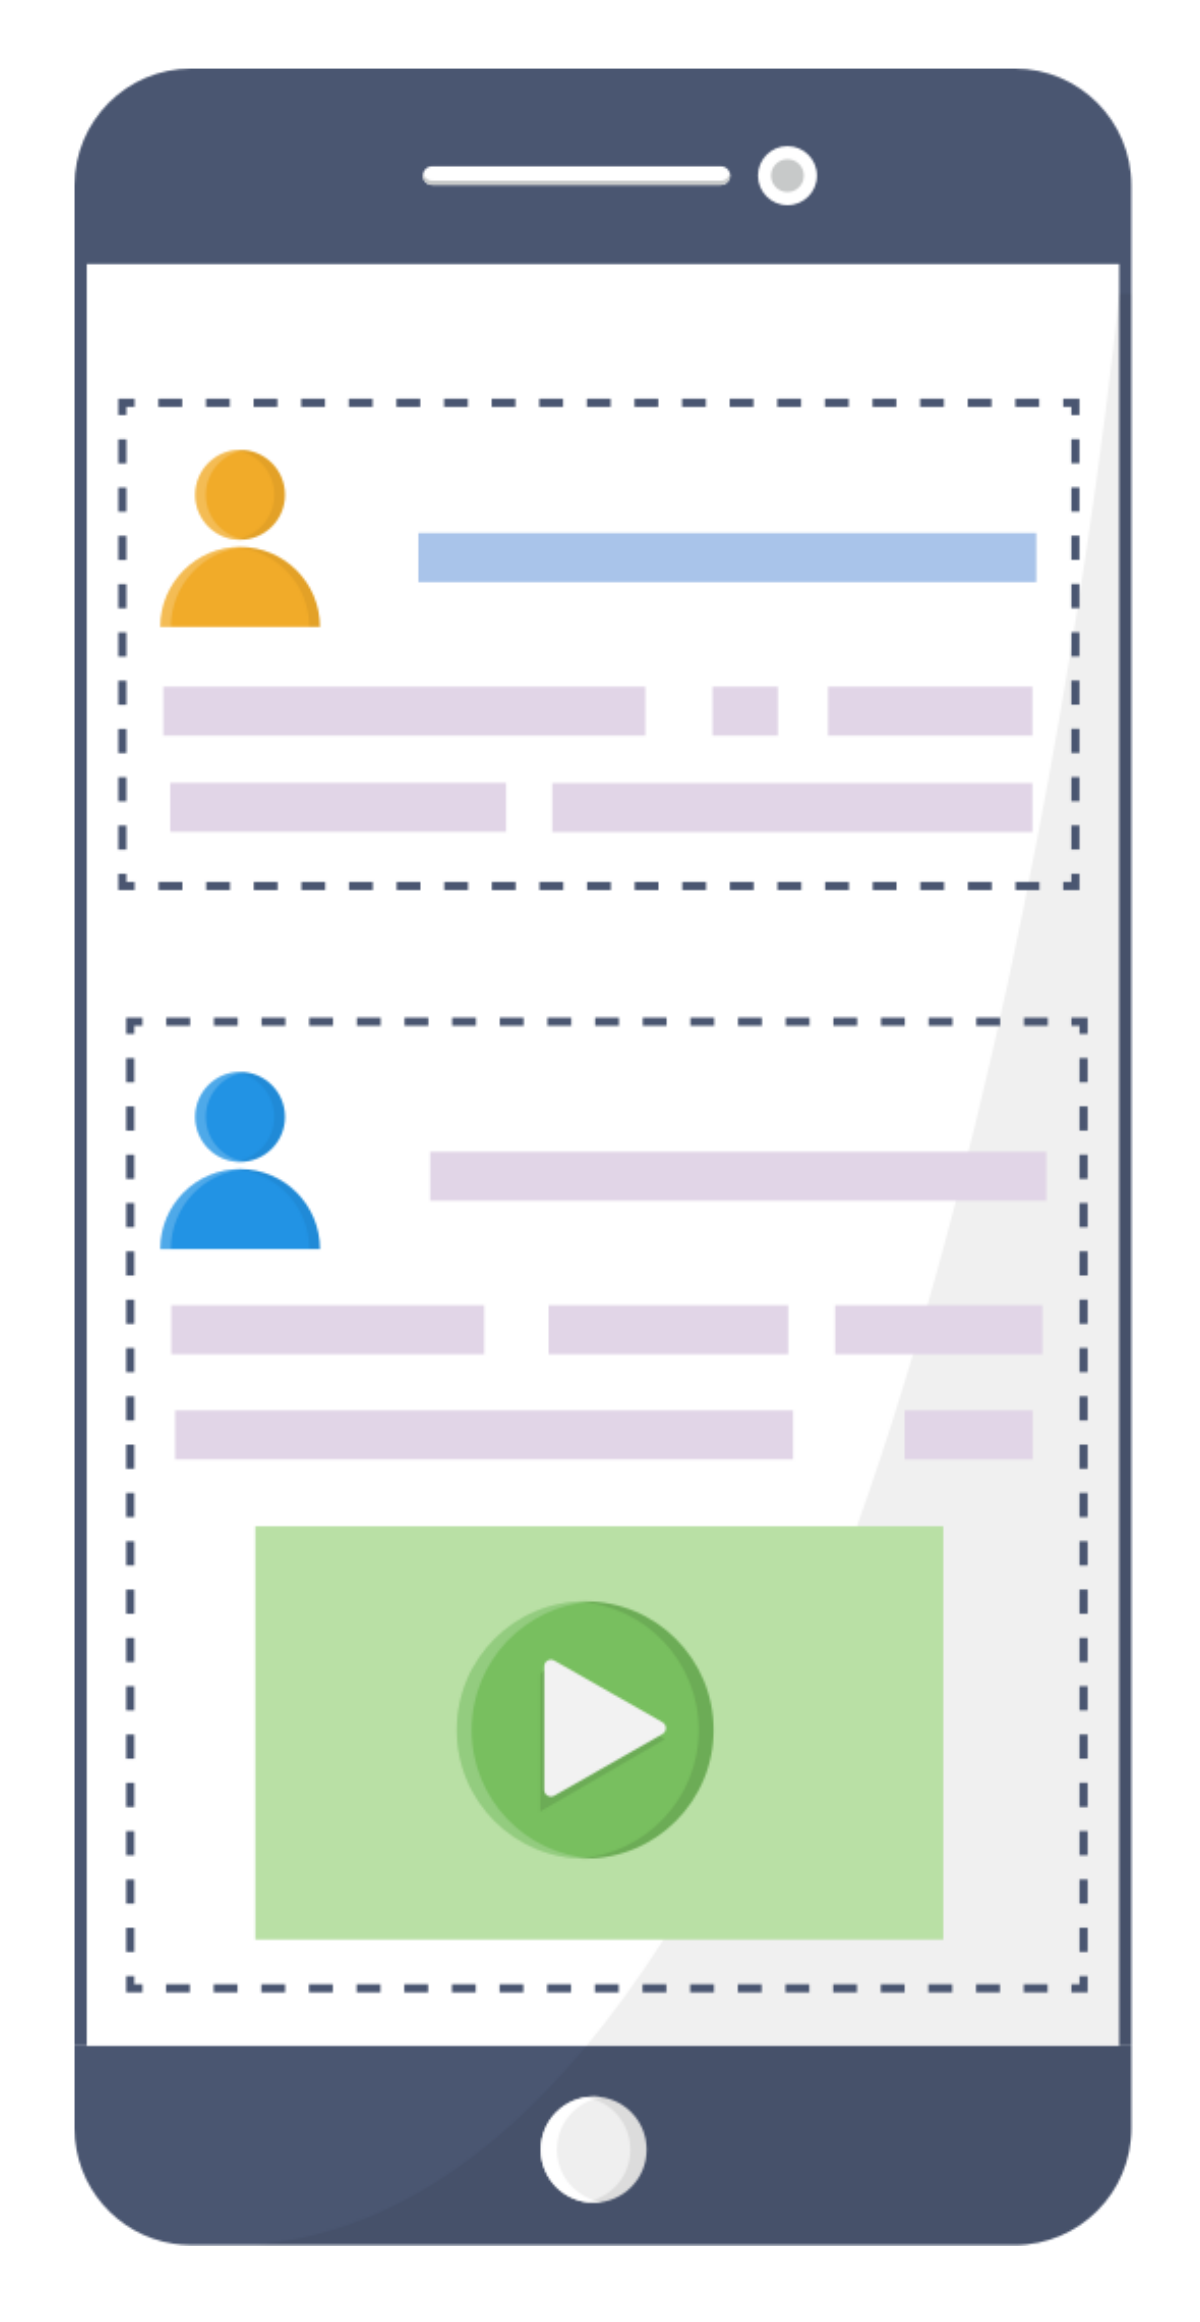
\includegraphics[width=0.15\textwidth]{Images/chapter_32/section_4943636425080832/5785281275756544.png}
 \caption{Newsfeeds on a mobile application}
\end{figure}

Now that we understand what a newsfeed is and the challenges it presents, we will begin by defining the system\textquotesingle s requirements.

\subsection{Requirements}\label{EHeloUisVUb5IvyBoxC18}
\\
To limit the scope of the problem, we'll focus on the following functional and non-functional requirements:

\subsubsection{Functional requirements}\label{_yo4W9pgjt1CFrVAZUbTv}

\begin{itemize}
\item
\protect\phantomsection\label{tndOLJ51LR_Z22onzECbH}
\textbf{Newsfeed generation:} The system will generate newsfeeds based on pages, groups, and followers that a user follows. A user may have many friends and followers. Therefore, the system should be capable of generating feeds from all friends and followers. The challenge here is that there is potentially a huge amount of content. Our system needs to decide which content to pick for the user and rank it further to decide which to show first.
\item
\protect\phantomsection\label{s0Df1u2Bu9BCUKs4cdcke}
\textbf{Newsfeed contents:} The newsfeed may contain text, images, and videos.
\item
\protect\phantomsection\label{qv-O7WeGAlWei8tp79G6f}
\textbf{Newsfeed display:} The system should affix new incoming posts to the newsfeed for all active users based on some ranking mechanism. Once ranked, we show content to a user with higher-ranked first.
\end{itemize}

\subsubsection{Non-functional requirements}\label{Yk89ZfRB_4WYYhRfwvki6}

\begin{itemize}
\item
\protect\phantomsection\label{ZL_UG12X7-Iq0C1Da_07h}
\textbf{Scalability:} Our proposed system should be highly scalable to support the ever-increasing number of users on any platform, such as Twitter, Facebook, and Instagram.
\item
\protect\phantomsection\label{K_x1dcLFJbFuUO-qIqH7S}
\textbf{Fault tolerance:}~As the system should be handling a large amount of data, therefore, partition tolerance (system availability in the event of network failure between the system's components) is necessary.
\item
\protect\phantomsection\label{2FhitDW1PT4TfB-fREaQK}
\textbf{Availability:} The service must be highly available to keep the users engaged with the platform. The system can compromise strong consistency for availability and fault tolerance, according to the PACELC theorem(The PACELC theorem is an extension of the CAP theorem that states, in the event of network Partition, one should choose between Availability or Consistency; else, choose between Latency and Consistency.).
\item
\protect\phantomsection\label{vdXEytb1i772djA9ZSONl}
\textbf{Low latency:} The system should provide newsfeeds in real-time. Hence, the maximum latency should not be greater than 2 seconds.
\end{itemize}
\\
These requirements, particularly scalability, need to be quantified. The process of resource estimation will help us understand the magnitude of traffic, storage, and server power needed

\subsection{Resource estimation}\label{kNIPR8-UqTn-HqJEJ50Mw}
\\
Let's assume the platform for which the newsfeed system is designed has 1 billion users per day, out of which, on average, 500 million are daily active users. Also , each user has 300 friends and follows 250 pages on average. Based on the assumed statistics, let's look at the traffic, storage, and server estimation.

\subsubsection{Traffic estimation}\label{gDv52qvIEas9go1133JX_}
\\
Let's assume that each daily active user opens the application (or social media page) 10 times a day. The total number of requests per day would be:\\
\strut \\
\protect\phantomsection\label{katex_inline_BmCFsJG0HqQ5yHRk99dOL}{{{\(500 M \times 10 = 5\)}}} billions request per day \protect\phantomsection\label{katex_inline_wfjU8pzxH-GVLVSbHQWr1}{{{\(\approx 58K\)}}} requests per second.

\begin{figure}[htbp]
 \centering
 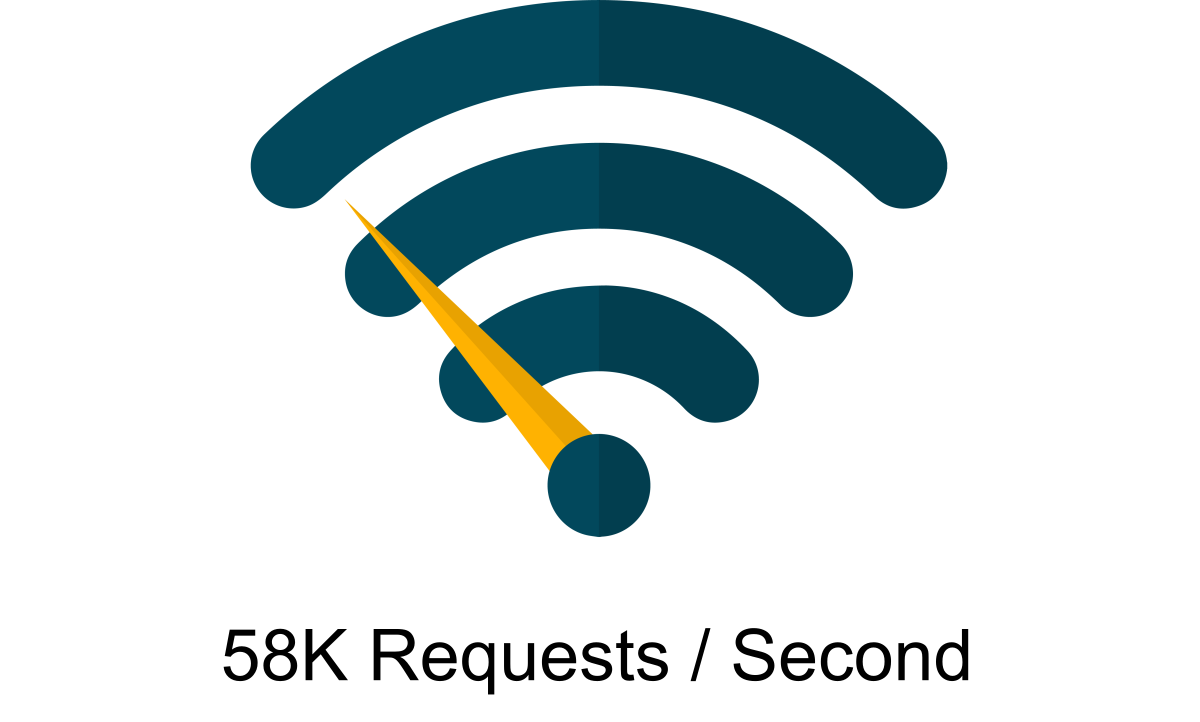
\includegraphics[width=0.15\textwidth]{Images/chapter_32/section_4943636425080832/6467035144126464.png}
 \caption{Traffic estimation for the newsfeed system}
\end{figure}

\subsubsection{Storage estimation}\label{K-rt1z93fS-bd3PcVn0FL}
\\
Let's assume that the feed will be generated offline and rendered upon a request. Also , we'll precompute the top 200 posts for each user. Let
's calculate storage estimates for users' metadata, posts containing text, and media content.

\begin{enumerate}
\item
\protect\phantomsection\label{TJMlRZxrWI10Cj2k567so}
\textbf{Users' metadata storage estimation:} Suppose the storage required for one user's metadata is 50 KB. For 1 billion users, we would need\protect\phantomsection\label{katex_inline_3Qomp1XEhamDi3r22CRxX}{{{\(1B\times 50KB = 50 TB\)}}}.\\
We can tweak the estimated numbers and calculate the storage for our desired numbers in the following calculator:
\end{enumerate}

\begin{enumerate}
\setcounter{enumi}{1}
\item
\protect\phantomsection\label{-SSUdAHgQskki9CxpJrNX}
\textbf{Textual post's storage estimation:} All posts could contain some text, we assume it's 5KB on average. The storage estimation for the top 200 posts for 500 million users would be:\\
\protect\phantomsection\label{katex_inline_ShHVRzY92Ete3CZoz2twg}{{{\(\text{200} \times \text{500M} \times \text{5 KB} = \text{0.5 PB}\)}}}
\item
\protect\phantomsection\label{18eTnq3yvfS1IMe8bTrV2}
\textbf{Media content storage estimate:} Along with text, a post can also contain media content. Therefore, we assume that \protect\phantomsection\label{katex_inline_SvjsF9KEybDtKu5jTD2Aq}{{{\(1/5th\)}}} posts have videos and \protect\phantomsection\label{katex_inline_x77cvq8s2aH5sfCjduPVY}{{{\(4/5th\)}}} include images. The assumed average image size is 200KB and the video size is 2MB.\\
Storage estimate for 200 posts of one user:\\
\protect\phantomsection\label{katex_inline_ZYFKrtPMggGpVNjelb4Yc}{{{\(\left( \text{200} \times \text{2 MB} \times \frac{1}{5} \right) + \left( \text{200} \times \text{200 KB} \times \frac{4}{5} \right) = \text{80 MB} + \text{32 MB} = \text{112 MB}\)}}}\\
Total storage required for 500 million users' posts: \protect\phantomsection\label{katex_inline_yyIWU2cYY39btmdx4GOcU}{{{\(\text{112 MB} \times \text{500M} = \text{56 PB}\)}}}\\
So we'll need at least 56PB of blob storage to store the media content.
\end{enumerate}

\begin{figure}[htbp]
 \centering
 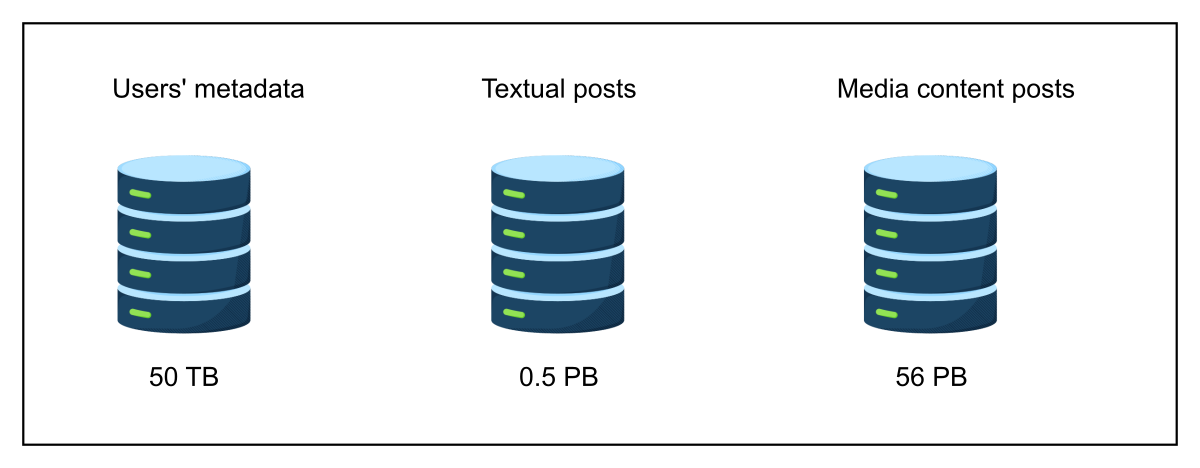
\includegraphics[width=0.5\textwidth]{Images/chapter_32/section_4943636425080832/6132432699785216.png}
 \caption{Storage required for 500 million active users per day (each with approx. 200 posts) by newsfeed system}
\end{figure}

\subsubsection{Number of servers estimation}\label{4Ixs0CWxKR90qAcxts6fa}
\\
Considering the above traffic, let's estimate the required number of servers during peak load. Recall that a typical server can serve 64,000 requests per second (RPS). Considering
\href{https://www.educative.io/courses/grokking-the-system-design-interview/put-back-of-the-envelope-numbers-in-perspective}{our assumption} of using~daily active users as a proxy for the number of requests per second for peak load times, we get 500 million requests per second. Then
, we use the following formula to calculate the number of servers:

\[
\text{Servers needed at peak load} = \frac{\text{Number of requests/second}}{\text{RPS of server}}
\]

\[
\text{Servers needed at peak load} = \frac{\text{500 million}}{\text{64,000}} = \text{7812.5} \approx \text{8K servers}
\]

\begin{figure}[htbp]
 \centering
 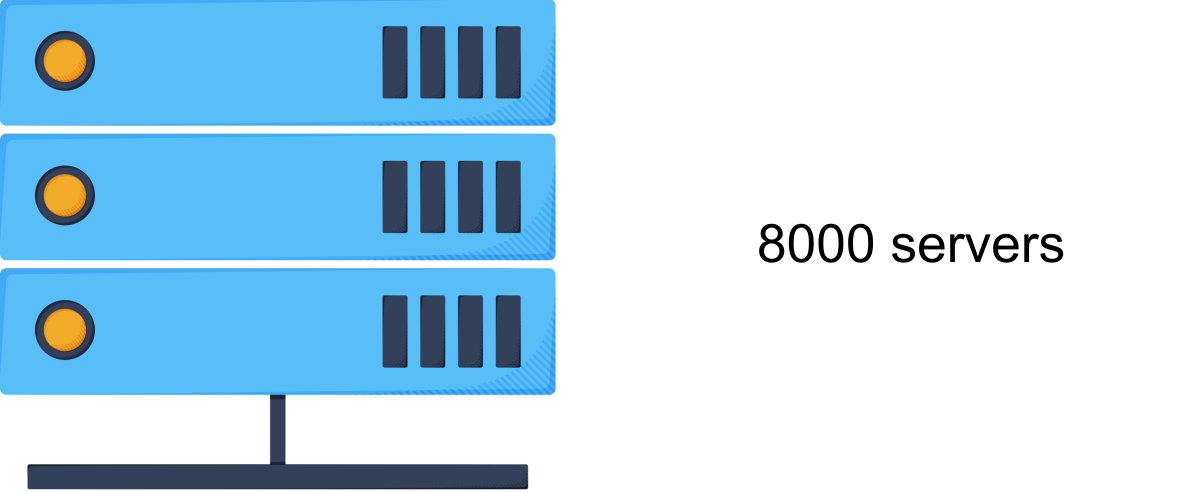
\includegraphics[width=0.5\textwidth]{Images/chapter_32/section_4943636425080832/5396674694742016.png}
 \caption{The number of servers required for the newsfeed system}
\end{figure}

Let\textquotesingle s review the essential building blocks needed to construct the newsfeed system.

\subsection{Building blocks we will use}\label{cw47UKTV0IEglcBnbZgFC}

The design of newsfeed system utilizes the following building blocks:

\begin{figure}[htbp]
 \centering
 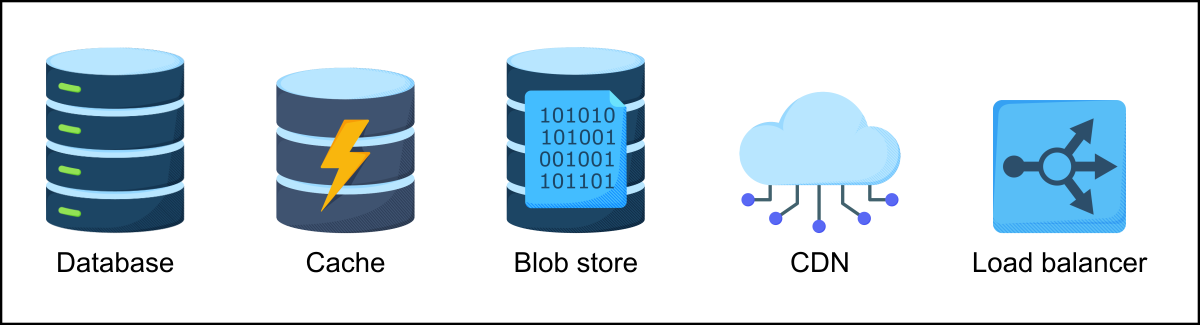
\includegraphics[width=0.5\textwidth]{Images/chapter_32/section_4943636425080832/5259969710915584.png}
 \caption{The building blocks to design a newsfeed system}
\end{figure}

\begin{itemize}
\item
\protect\phantomsection\label{tACpOS_sOzIy0HUFkqY9R}
\href{https://www.educative.io/courses/grokking-the-system-design-interview/introduction-to-databases}{\textbf{Database(s)}} is required to store the posts from different entities and the generated personalized newsfeed. It is also used to store users' metadata and their relationships with other entities, such as friends and followers.
\item
\protect\phantomsection\label{IsKAuDR8aMdMK_yEFMElO}
\href{https://www.educative.io/courses/grokking-the-system-design-interview/system-design-the-distributed-cache}{\textbf{Cache}} is an important building block to keep the frequently accessed data, whether posts and newsfeeds or users' metadata.
\item
\protect\phantomsection\label{s9bJvdFVkBytOc7moJK6_}
\href{https://www.educative.io/courses/grokking-the-system-design-interview/system-design-a-blob-store}{\textbf{Blob storage}} is essential to store media content, for example, images and videos.
\item
\protect\phantomsection\label{LMq5t8kF8-Ta78i37w3gh}
\href{https://www.educative.io/courses/grokking-the-system-design-interview/system-design-the-content-delivery-network-cdn}{\textbf{CDN}} effectively delivers content to end-users reducing delay and burden on back-end servers.
\item
\protect\phantomsection\label{_Y0ThHiJYlqUjcAeDyK7r}
\href{https://www.educative.io/courses/grokking-the-system-design-interview/introduction-to-load-balancers}{\textbf{Load balancers}} are necessary to distribute millions of incoming clients' requests for newsfeed among the pool of available servers.
\end{itemize}
\\
Having identified the requirements and important building blocks, let's discuss the high-level and detailed design of a newsfeed system.

\subsection{High-level design of a newsfeed system}\label{XeLx1fUSifJdnPrmeF7nS}
\\
Primarily, the newsfeed system is responsible for the following two tasks:

\begin{enumerate}
\item
\protect\phantomsection\label{UgxDGMng5A1IqBq1U0Sf7}
\textbf{Feed generation:} The newsfeed is generated by aggregating friends' and followers' posts (or feed items) based on some ranking mechanism.
\item
\protect\phantomsection\label{RPlqet6aK7WJ0Pc_M09wJ}
\textbf{Feed publishing:} When a feed is published, the relevant data is written into the cache and database. This data could be textual or any media content. A post containing the data from friends and followers is populated to a user's newsfeed.
\end{enumerate}
\\
Let's move to the high-level design of our newsfeed system. It consists of the above two essential parts, shown in the following figure:

\begin{figure}[htbp]
 \centering
 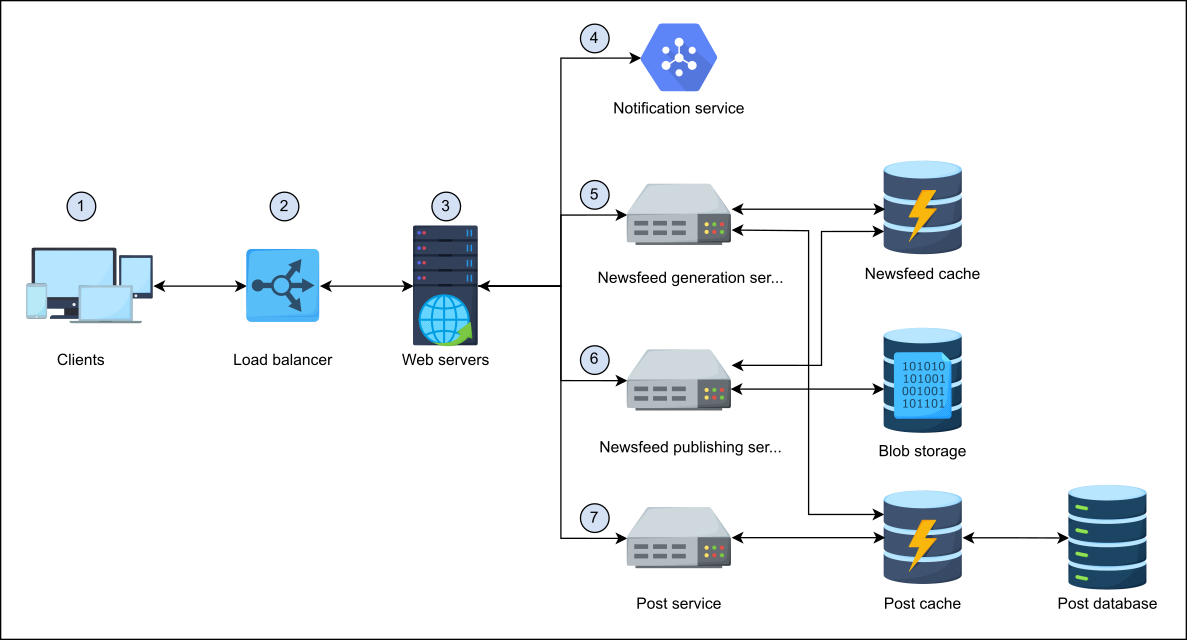
\includegraphics[width=0.5\textwidth]{Images/chapter_32/section_4943636425080832/5546678507929600.png}
 \caption{High-level design of the Newsfeed system}
\end{figure}

Let's discuss the main components shown in the high-level design:

\begin{enumerate}
\item
\protect\phantomsection\label{mAgi_U1auXRpDujzJuUy-}
\textbf{User(s):} Users can make a post with some content or request their newsfeed.
\item
\protect\phantomsection\label{rKis8I6Z2ABmKpGunXLRW}
\textbf{Load balancer:} It redirects traffic to one of the web servers.
\item
\protect\phantomsection\label{2J-DUi2cM5VKBGyjOCsI_}
\textbf{Web servers:} The web servers encapsulate the back-end services and work as an intermediate layer between users and various services. Apart from enforcing authentication and rate-limiting, web servers are responsible to redirect traffic to other back-end services.
\item
\protect\phantomsection\label{vrEjRA2grALalvzc9RFf2}
\textbf{Notification service:} It informs the newsfeed generation service whenever a new post is available from one's friends or followers, and sends a push notification.
\item
\protect\phantomsection\label{MIqTOeJZX9_uI_MMUkUY6}
\textbf{Newsfeed generation service:} This service generates newsfeeds from the posts of followers/friends of a user and keeps them in the newsfeed cache.
\item
\protect\phantomsection\label{UQ2t3KAi9SYv5iaKGqRVD}
\textbf{Newsfeed publishing service:} This service is responsible for publishing newsfeeds to a users' timeline from the newsfeed cache. It also appends a thumbnail of the media content from the blob storage and its link to the newsfeed intended for a user.
\item
\protect\phantomsection\label{woKY-I7V0-bdSBwfRSGAK}
\textbf{Post-service:} Whenever a user requests to create a post, the post-service is called, and the created post is stored on the post database and corresponding cache. The media content in the post is stored in the blob storage.
\end{enumerate}
\\
Newsfeeds often grapple with the issue of misinformation spread. What are two design-level interventions you could implement to help mitigate this problem?

\textbf{Question:}

Design strategies to combat misinformation in a newsfeed

\textbf{Reference Answer:}

Flag or downrank content with suspicious origins or lacking verification. Collaborate with fact-checking organizations to validate information.

To translate this high-level diagram into a working system, we must define the contracts between its services. This brings us to the API design.

\subsection{API design}\label{FXhjRWzLLhlLJ1SQU3pwH}
\\
APIs are the primary ways for clients to communicate with servers. Usually , newsfeed APIs are HTTP-based that allow clients to perform actions, including posting a status, retrieving newsfeeds, adding friends, and so on. We aim to generate and get a user's newsfeed; therefore, the following APIs are essential:

\subsubsection{Generate the user's newsfeed}\label{0L1YbHPovGkkO8Op1taAF}
\\
The following API is used to generate a user's newsfeed:

\begin{lstlisting}[language=JavaScript]
generateNewsfeed(user_id)
\end{lstlisting}

This API takes users' IDs, and determines their friends and followers. This API generates newsfeeds that consist of several posts. Since internal system components use this API, therefore, it can be called offline to pre-generate newsfeeds for users. The pre-generated newsfeeds are stored on persistent storage and associated cache.
\\
The following parameter is used in this API call:

\begin{table}[htbp]
\centering
\small
\adjustbox{max width=\textwidth}{
\begin{tabular}{|p{0.208\textwidth}|p{0.742\textwidth}|}
\hline
\textbf{Parameter} & \textbf{Description} \\
\hline
\hline
\texttt{user\_id} & A unique identification of the user for whom the newsfeed is generated. \\
\hline
\end{tabular}
}
\end{table}

\subsubsection{Get the user's newsfeed}\label{ZA6uFr5Z4Gt44AJ6ZT-9o}
\\
The following API is used to get a user's newsfeed:

\begin{lstlisting}[language=JavaScript]
getNewsfeed(user_id, count)
\end{lstlisting}

The \texttt{getNewsfeed(.)} API call returns a JSON object consisting of a list of posts.
\\
The following parameters are used for this API:

\begin{table}[htbp]
\centering
\small
\adjustbox{max width=\textwidth}{
\begin{tabular}{|p{0.208\textwidth}|p{0.742\textwidth}|}
\hline
\textbf{Parameter} & \textbf{Description} \\
\hline
\hline
\texttt{user\_id} & A unique identification of the user for whom the system will fetch the newsfeed. \\
\hline
\texttt{count} & The number of feed items (posts) that will be retrieved per request. \\
\hline
\end{tabular}
}
\end{table}

\subsection{Storage schema}\label{mQbPy8Idt_sUBJEu8nEFq}
\\
The database relations for the newsfeed system are as follows:

\begin{itemize}
\item
\protect\phantomsection\label{HYIRwZhydMG8ZPAtcFNeg}
\textbf{User:} This relation contains data about a user. A user can also be a follower or friend of other users.
\item
\protect\phantomsection\label{4pKdxiRVHtV84hMGSI-RV}
\textbf{Entity:} This relation stores data related to any entity, such as pages, groups, and so on.
\item
\protect\phantomsection\label{eDSCVQ0JXdy4TStSuB_cB}
\textbf{Feed\_item:} The data about posts created by users is stored in this relation.
\item
\protect\phantomsection\label{U9ydCcCndGjuvp5MPF2gj}
\textbf{Media:} The information about the media content is stored in this relation.
\end{itemize}

\begin{figure}[htbp]
 \centering
 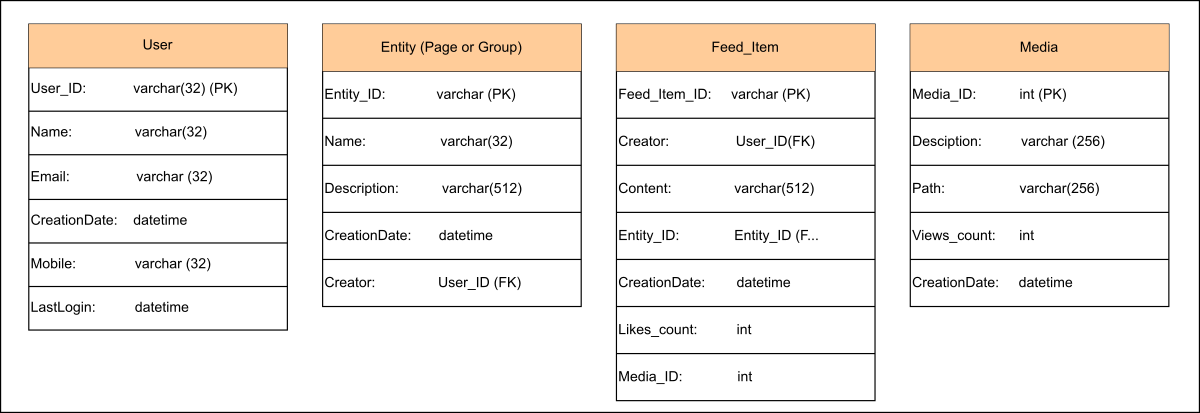
\includegraphics[width=0.5\textwidth]{Images/chapter_32/section_4943636425080832/6500327381794816.png}
 \caption{The database schema for the newsfeed system}
\end{figure}

The user and post data is structured, so we will use SQL-based databases to store it. We use a graph database to store relationships between users, friends, and followers. For this purpose, we follow the property graph model(In the property graph model, connections (edges) carry a name and some properties that represent the relationship between two entities.). We can think of a graph database consisting of two relational tables:

\begin{enumerate}
\item
\protect\phantomsection\label{OP0m5x3lZVlsaqJTpWiPs}
For vertices that represent users
\item
\protect\phantomsection\label{YuIQqVgDWrcc2WdaEOMLd}
For edges that denotes relationships among them
\end{enumerate}
\\
Therefore, we follow a relational schema for the graph store, as shown in the following figure. The schema uses the PostgreSQL JSON data type to store the properties of each vertex (user) or edge (relationship).
\\
An alternative representation of a \textbf{User} can be shown in the graph database below. Where the Users\_ID remains the same and attributes are stored in a JSON file format.

\begin{figure}[htbp]
 \centering
 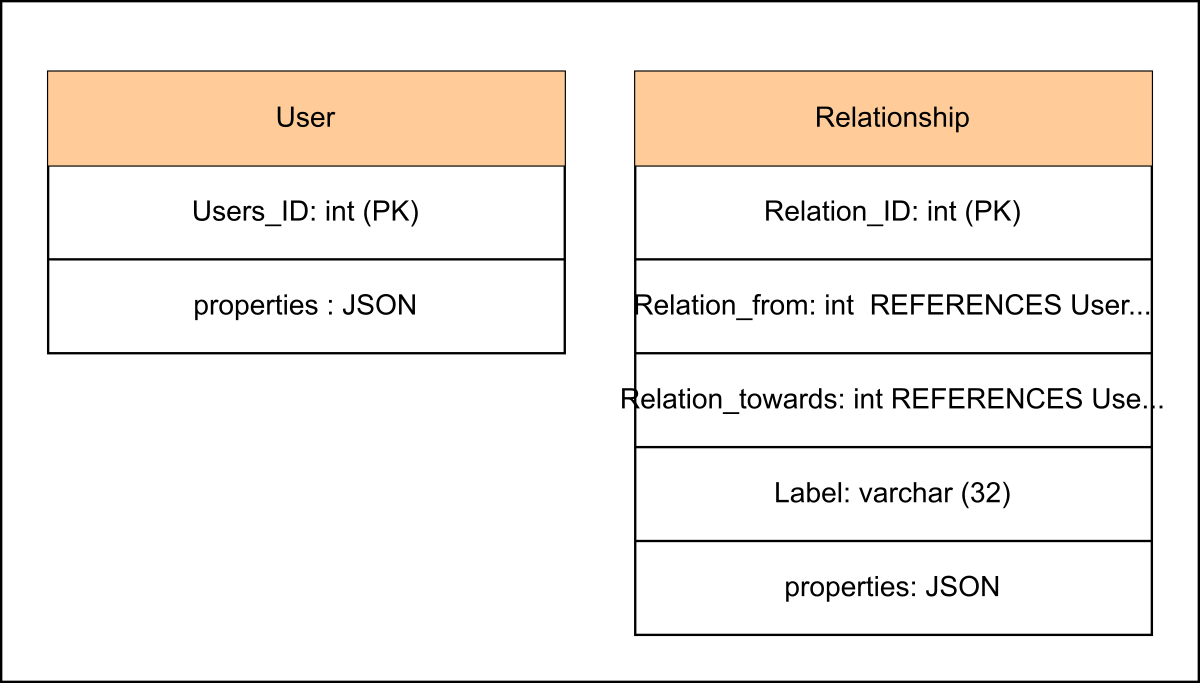
\includegraphics[width=0.5\textwidth]{Images/chapter_32/section_4943636425080832/5425188015702016.png}
 \caption{Schema of the graph database to hold relationships between users}
\end{figure}

The following figure demonstrates how a graph can be represented using the relational schema:

\begin{figure}[htbp]
 \centering
 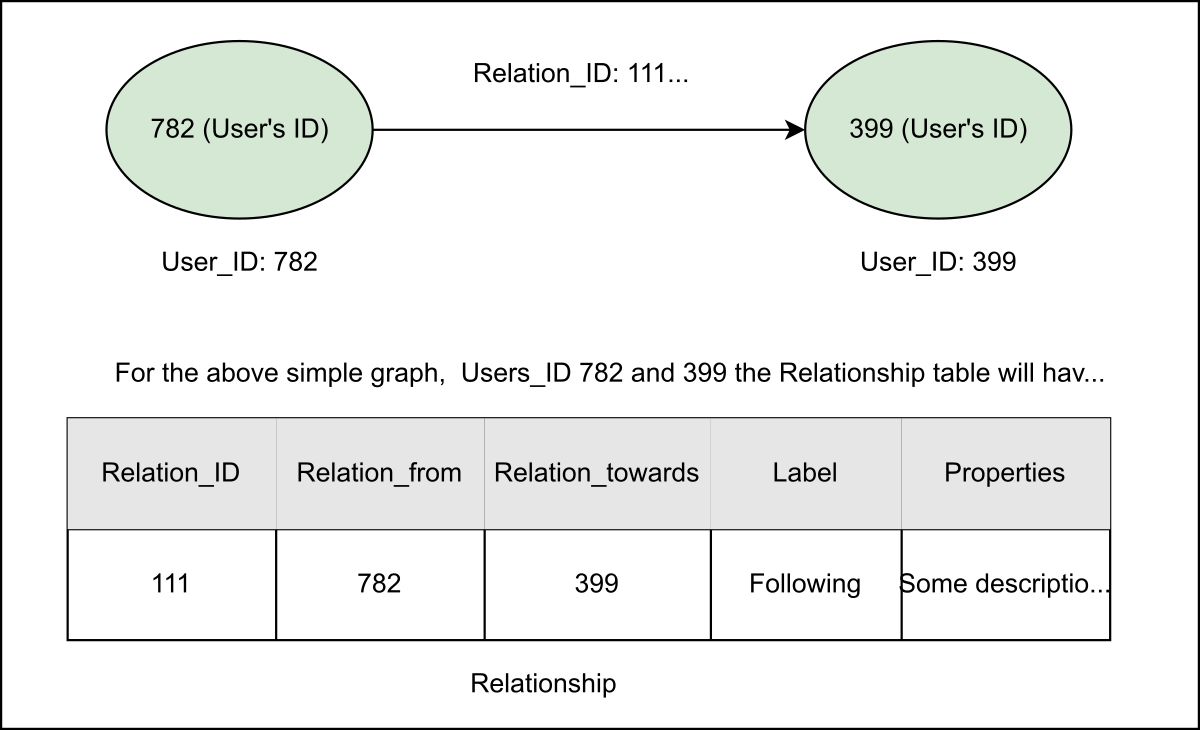
\includegraphics[width=0.5\textwidth]{Images/chapter_32/section_4943636425080832/6365445471600640.png}
 \caption{A graph between two users consisting of two vertices and an edge}
\end{figure}

With the foundational pieces of architecture and data structure in place, we can now zoom in. The section below explores the inner workings and logic of the core services in our detailed design.

\subsection{Detailed design}\label{3pYLspEvwJaLhEZK2hYwg}
\\
As discussed earlier, there are two parts of the newsfeed system; newsfeed publishing and newsfeed generation. Therefore, we'll discuss both parts, starting with the newsfeed generation service.

\subsubsection{The newsfeed generation service}\label{Ju1rYQo9daV5SEJ4UKG3C}
\\
Newsfeed is generated by aggregated posts (or feed items) from the user's friends, followers, and other entities (pages and groups).
\\
In our proposed design, the \textbf{newsfeed generation service} is responsible for generating the newsfeed. When a request from a user (say Alice) to retrieve a newsfeed is received at the web servers, the web server either:

\begin{itemize}
\item
\protect\phantomsection\label{NcQZhI0yfI64iq2As-_6R}
Calls the newsfeed generation service to generate feeds because some users don't often visit the platform, so their feeds are generated on their request.
\item
\protect\phantomsection\label{9_eI6gGqUaKuN5uRRlv5R}
It fetches the pre-generated newsfeed for active users who visit the platform frequently.
\end{itemize}
\\
The following steps are performed in sequence to generate a newsfeed for Alice:

\begin{enumerate}
\item
\protect\phantomsection\label{ulS4HqgVr-ZoEzRkOrvhq}
The newsfeed generation service retrieves IDs of all users and entities that Alice follows from the graph database.
\item
\protect\phantomsection\label{L2Ck54v7WWBuyPf1FLu8n}
When the IDs are retrieved from the graph database, the next step is to get their friends' (followers and entities) information from the user cache, which is regularly updated whenever the \textbf{users database} gets updated/modified.
\item
\protect\phantomsection\label{izTPAVJPAThOS9vExbvxK}
In this step, the service retrieves the latest, most popular, and relevant posts for those IDs from the post cache. These are the posts that we might be able to display on Alice's newsfeed.
\item
\protect\phantomsection\label{1BQ7DiK3VqIDb2v-LT8Qx}
The \textbf{ranking service} ranks posts based on their relevance to Alice. This represents Alice's current newsfeed.
\item
\protect\phantomsection\label{7viFEfH7R6wNj_IJ-xRp3}
The newsfeed is stored in the newsfeed cache from which the top N posts are published to Alice's timeline. (The publishing process is discussed in detail in the following section.)
\item
\protect\phantomsection\label{YF-qhUk1Y7AUOv66l01_D}
In the end, whenever Alice reaches the end of her timeline, the next top N posts are fetched to her screen from the newsfeed cache.
\end{enumerate}
\\
The process is illustrated in the following figure:

\begin{figure}[htbp]
 \centering
 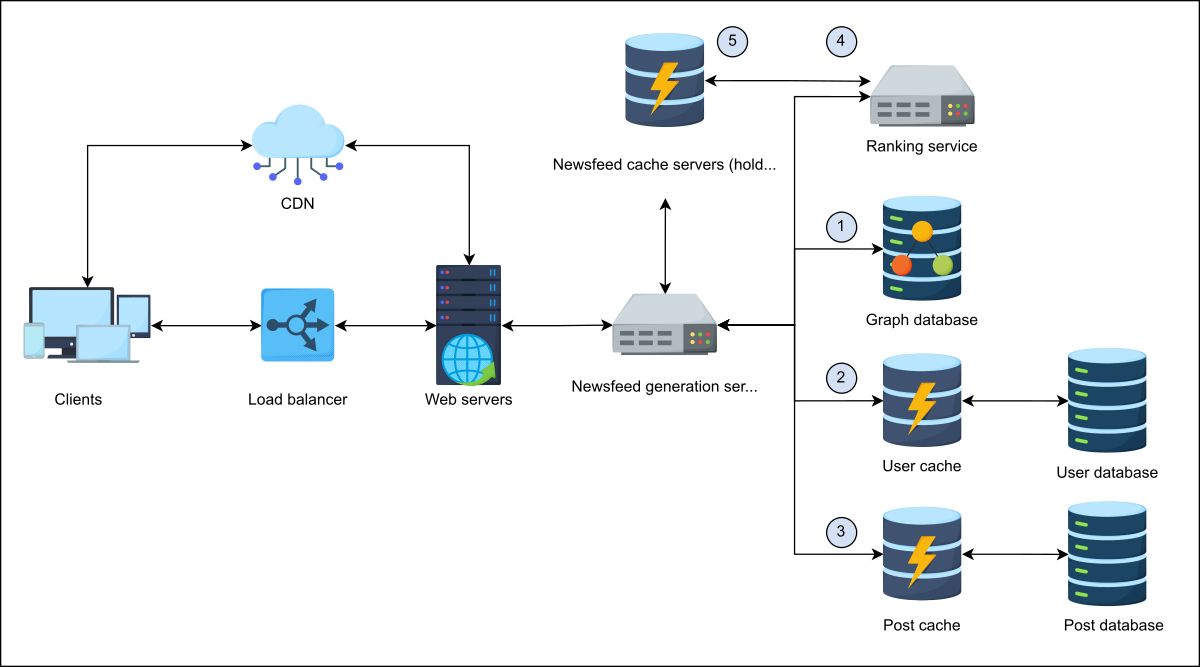
\includegraphics[width=0.5\textwidth]{Images/chapter_32/section_4943636425080832/5067718384812032.png}
 \caption{Working of the newsfeed generation service}
\end{figure}

\begin{quote}
\textbf{Quiz:}
\textbf{Question 1:} The creation and storage of newsfeeds for each user in the cache requires an enormous amount of memory (step 5 in the above section). Is there any way to reduce this memory consumption?
\textbf{Answer:} A more memory-efficient approach is to store an index that maps each

`User\_ID` to a list of their recent Post\_IDs. When a user requests their newsfeed, the system retrieves the list of users they follow, fetches the recent `Post\_IDs` for each of those users using the index,
pulls the corresponding post content from the database, and then merges and sorts the results to generate the final feed. This avoids the need to precompute and store full feeds for every user while still allowing efficient on-demand feed generation.
\end{quote}

\subsubsection{The newsfeed publishing service}\label{bkVefnPzktQAlX2MBT2dG}
\\
At this stage, the newsfeeds are generated for users from their respective friends, followers, and entities, and are stored in the form of \textless{Post\_ID,\ User\_ID\textgreater{}} in the news feed cache.
\\
Now the question is how the newsfeeds generated for Alice will be published to her timeline?
\\
The \textbf{newsfeed publishing service} fetches a list of post IDs from the newsfeed cache. The data fetched from the newsfeed cache is a tuple of post and user IDs, that is, \textless{Post\_ID,\ User\_ID\textgreater{}}. Therefore, the complete data about posts and users is retrieved from the users and posts cache to create an entirely constructed newsfeed.
\\
In the last step, the fully constructed newsfeed is sent to the client (Alice) using one of the fan-out approachesfanout. The popular newsfeed and media content are also stored in CDN for fast retrieval.

Suppose if our service receives billions of requests at once and the system starts generating live newsfeeds. This situation would put an enormous number of users on hold and could crash servers. To avoid this, we can assign dedicated servers that will continuously rank and generate newsfeeds and store them in the newsfeed database and memory. Therefore, upon a request for new posts from a user, our system will provide the pre-generated feeds.

\begin{figure}[htbp]
 \centering
 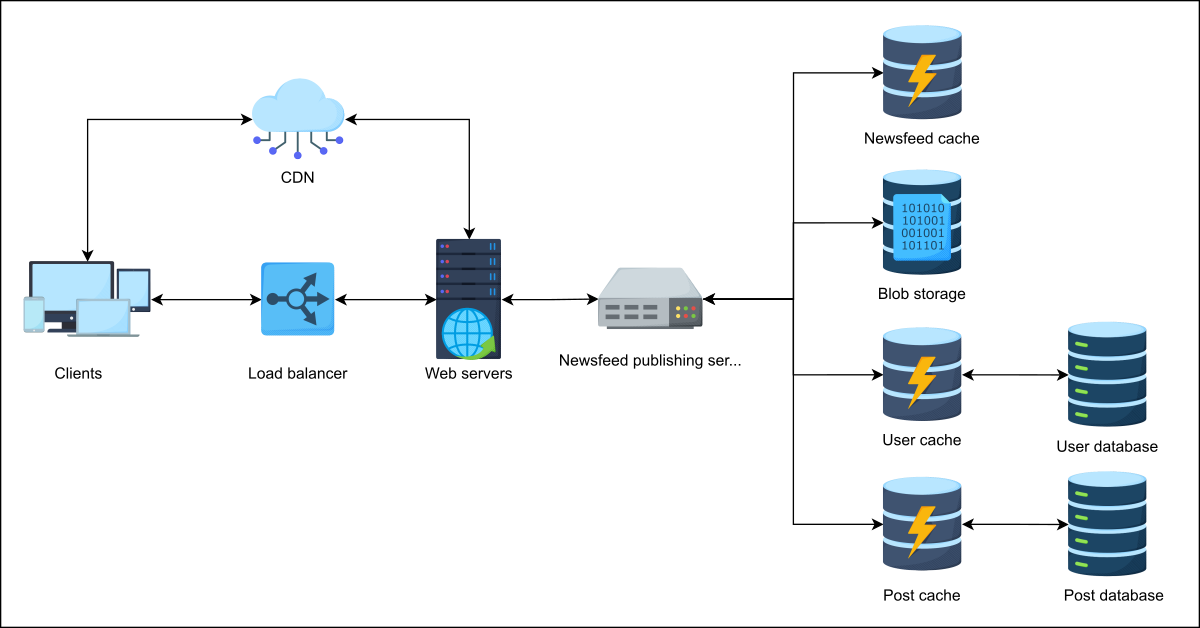
\includegraphics[width=0.5\textwidth]{Images/chapter_32/section_4943636425080832/6376947125190656.png}
 \caption{The newsfeed publishing service in action}
\end{figure}

\begin{quote}
\textbf{Quiz:}
\textbf{Question 1:} How is the newsfeed of the friends and followers updated when a user creates a new post?
\textbf{Answer:} When a user, say Bob, creates a new post, it is stored in the post database and cache. In the next step, the **newsfeed generation service** generates a newsfeed for Bob's friends and followers, and the newsfeed cache is updated. The updated newsfeed is delivered to the corresponding users on the next page/screen refresh event.
\end{quote}

\subsubsection{The newsfeed ranking service}\label{iXulFF0m3LTkGbxrDSTkk}
\\
Often, we see the relevant and important posts at the top of our newsfeeds whenever we log in to our social media accounts. This ranking involves multiple advanced ranking and recommendation algorithms.
\\
In our design, the \textbf{newsfeed ranking service} consists of these algorithms working on various features, such as a user's past history, likes, dislikes, comments, clicks, and many more. These algorithms also perform the following functions:

\begin{itemize}
\item
\protect\phantomsection\label{dEa_D9y3KZNipQsDylFGj}
Select ``candidates'' posts to show in a newsfeed.
\item
\protect\phantomsection\label{7U09Q_zcExorAqUHsLPrV}
Eliminate posts including misinformation or clickbait from the candidate posts.
\item
\protect\phantomsection\label{gk0wL3n9oF-l-DSa89CDY}
Create a list of friends a user frequently interacts with.
\item
\protect\phantomsection\label{lBQ-LToHQhLbjmx6A-DmA}
Choose topics on which a user spent more time.
\end{itemize}
\\
The ranking system considers all the above points to predict relevant and important posts for a user.

\begin{figure}[htbp]
 \centering
 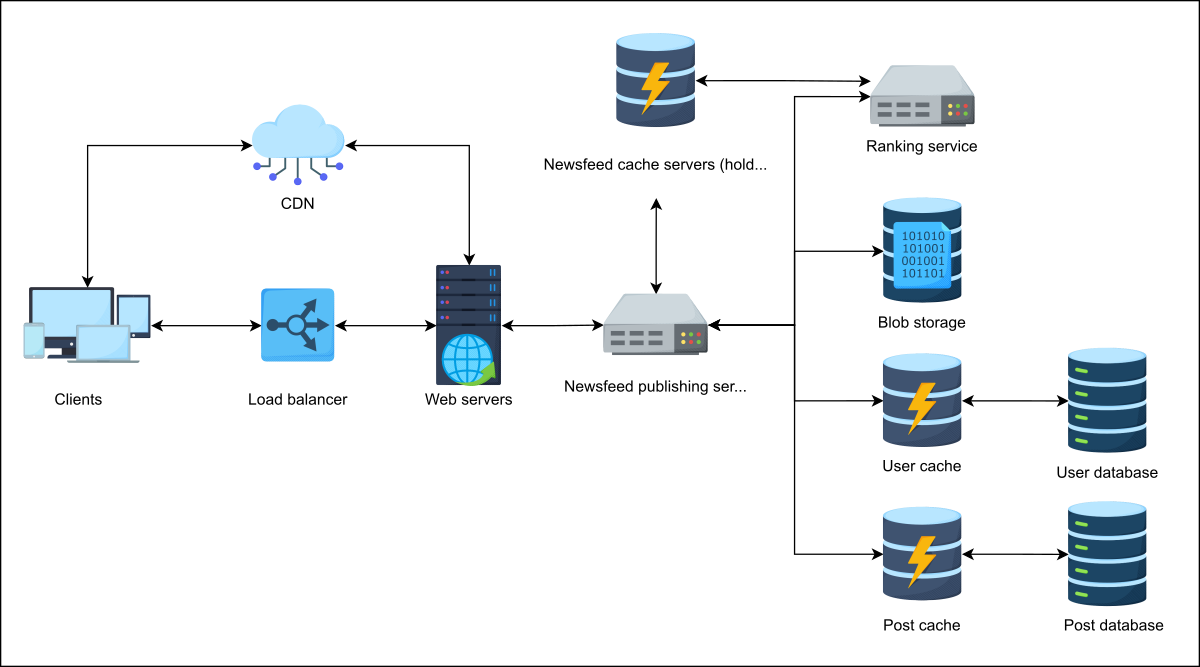
\includegraphics[width=0.5\textwidth]{Images/chapter_32/section_4943636425080832/6181045311766528.png}
 \caption{Working of the newsfeed generation service}
\end{figure}

\subsubsection{Post ranking and newsfeed construction}\label{W3e335yqqT15pzXI3r7zr}
\\
The post database contains posts published by different users. Assume that there are 10 posts in the database published by 5 different users. We aim to rank only 4 posts out of 10 for a user (say Bob) who follows those five different users. We perform the following to rank each post and create a newsfeed for Bob:

\begin{enumerate}
\item
\protect\phantomsection\label{VZYQfRRx7qD45sVSBtk1B}
Various features such as likes, comments, shares, category, duration, etc, and so on, are extracted from each post.
\item
\protect\phantomsection\label{kVwom7qKbSDz56oCfdoT6}
Based on Bob's previous history, stored in the \textbf{user database}, the relevance is calculated for each post via different ranking and machine learning algorithms.
\item
\protect\phantomsection\label{71uXaNX-1GMOT0N22i5yf}
A relevance score is assigned, say from 1 to 5, where 1 shows the least relevant post and 5 means a highly relevant post.
\item
\protect\phantomsection\label{YWePvEjmrsGWJGpzgEeLm}
The top 4 posts are selected out of 10 based on the assigned scores.
\item
\protect\phantomsection\label{0O2g3ogSjkilrT5jJMj2s}
The top 4 posts are combined and presented on Bob's timeline in decreasing order of the score assigned.
\end{enumerate}
\\
The following figure shows the top 4 posts published on Bob's timeline:

\begin{figure}[htbp]
 \centering
 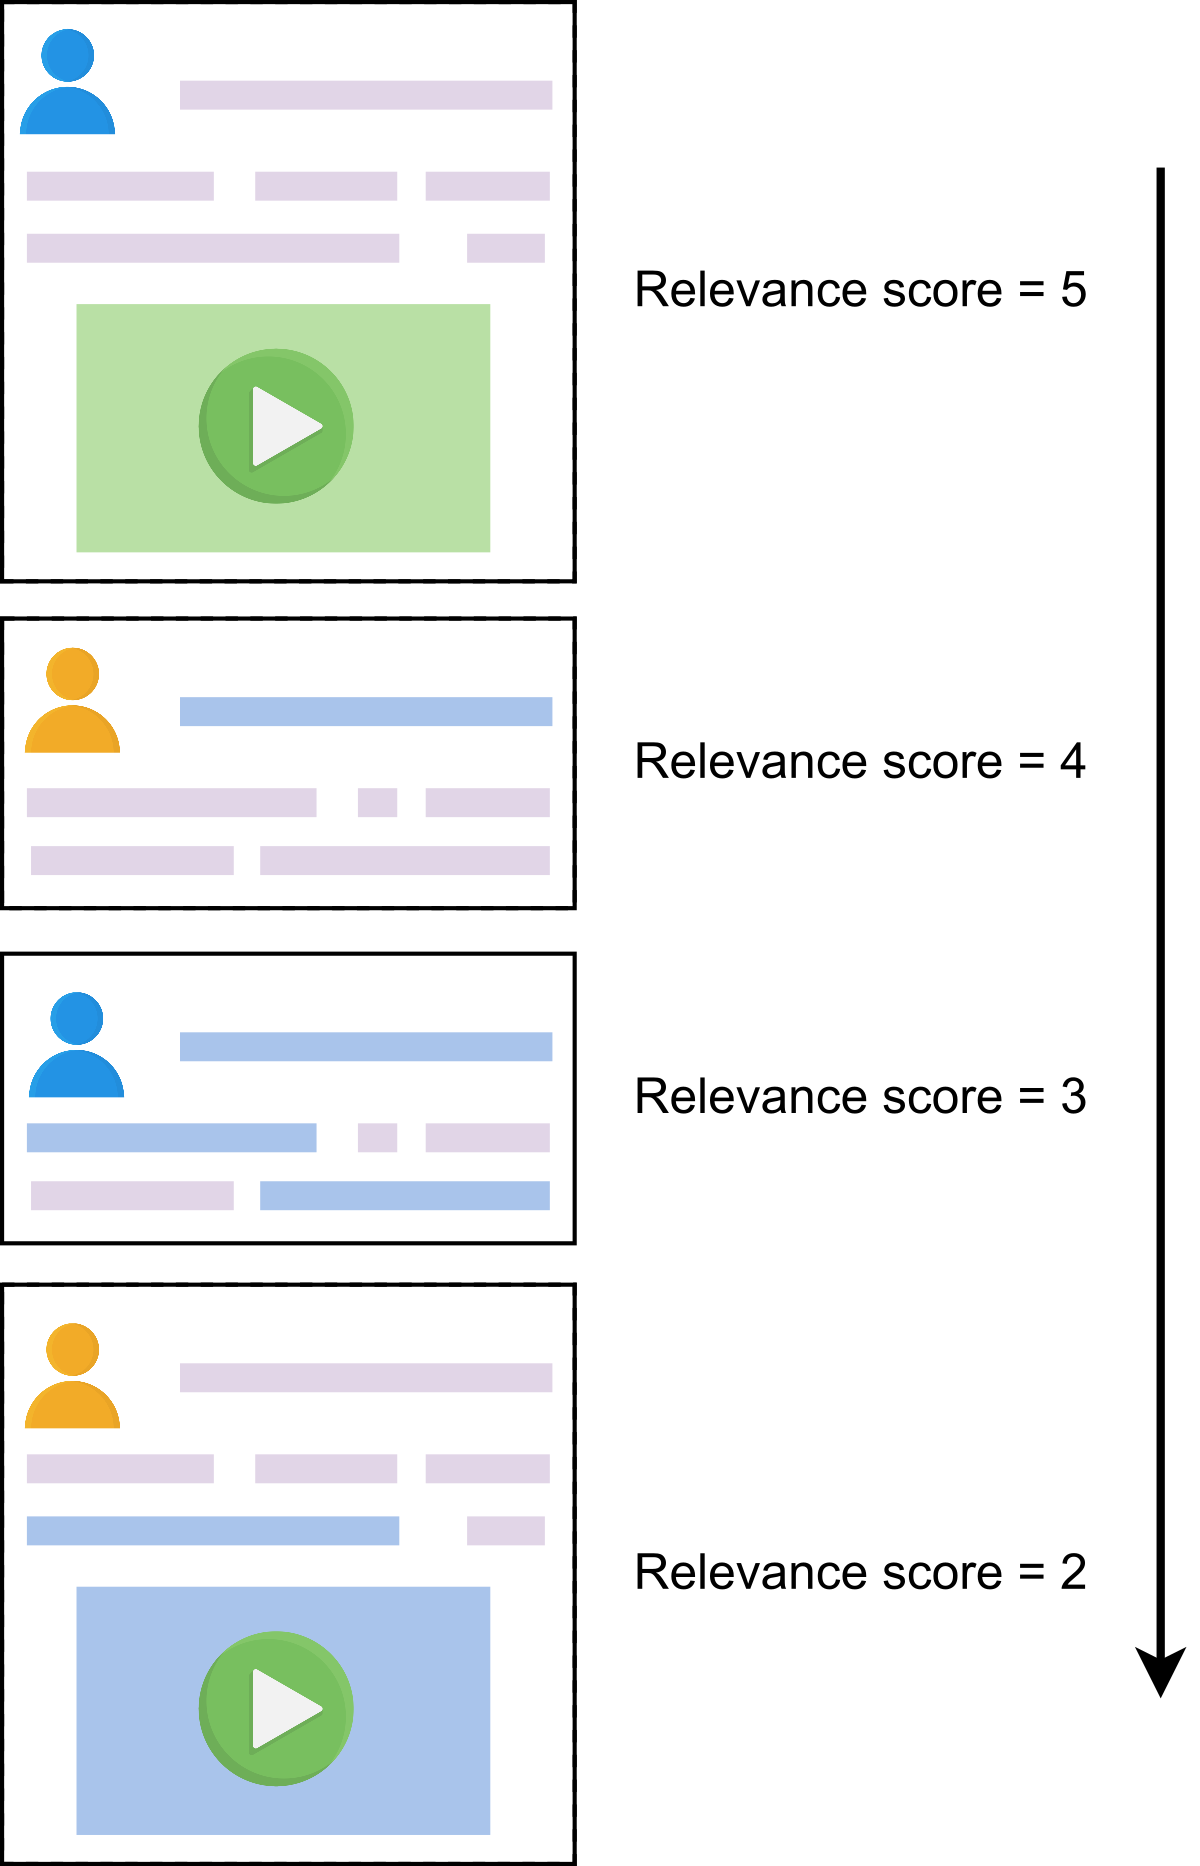
\includegraphics[width=0.15\textwidth]{Images/chapter_32/section_4943636425080832/5499205737250816.png}
 \caption{A newsfeed consisting of top 4 posts based on the relevance scores}
\end{figure}

Newsfeed ranking with various machine learning and ranking algorithms is a computationally intensive task. In our design, the \textbf{ranking service} ranks posts and constructs newsfeeds. This service consists of big-data processing systems that might utilize specialized hardware like graphics processing units (GPUs) and tensor processing units (TPUs).

\begin{quote}
\textbf{Note: According to Facebook:}
\\
``For each person on Facebook, we need to evaluate thousands of features to determine what that person might find most relevant to predict what each of those people wants to see in their feed.''
\\
This implies that we need enormous computational power and sophisticated learning algorithms to incorporate all the features to get good quality feed in a reasonably short time.
\end{quote}

Now it is time to synthesize this knowledge and see how all the components fit together in a single, comprehensive architecture.

\subsection{Putting everything together}\label{mW3xWJF51STLiu3kv_pfd}
\\
The following figure combines all the services related to the detailed design of the newsfeed system:

\begin{figure}[htbp]
 \centering
 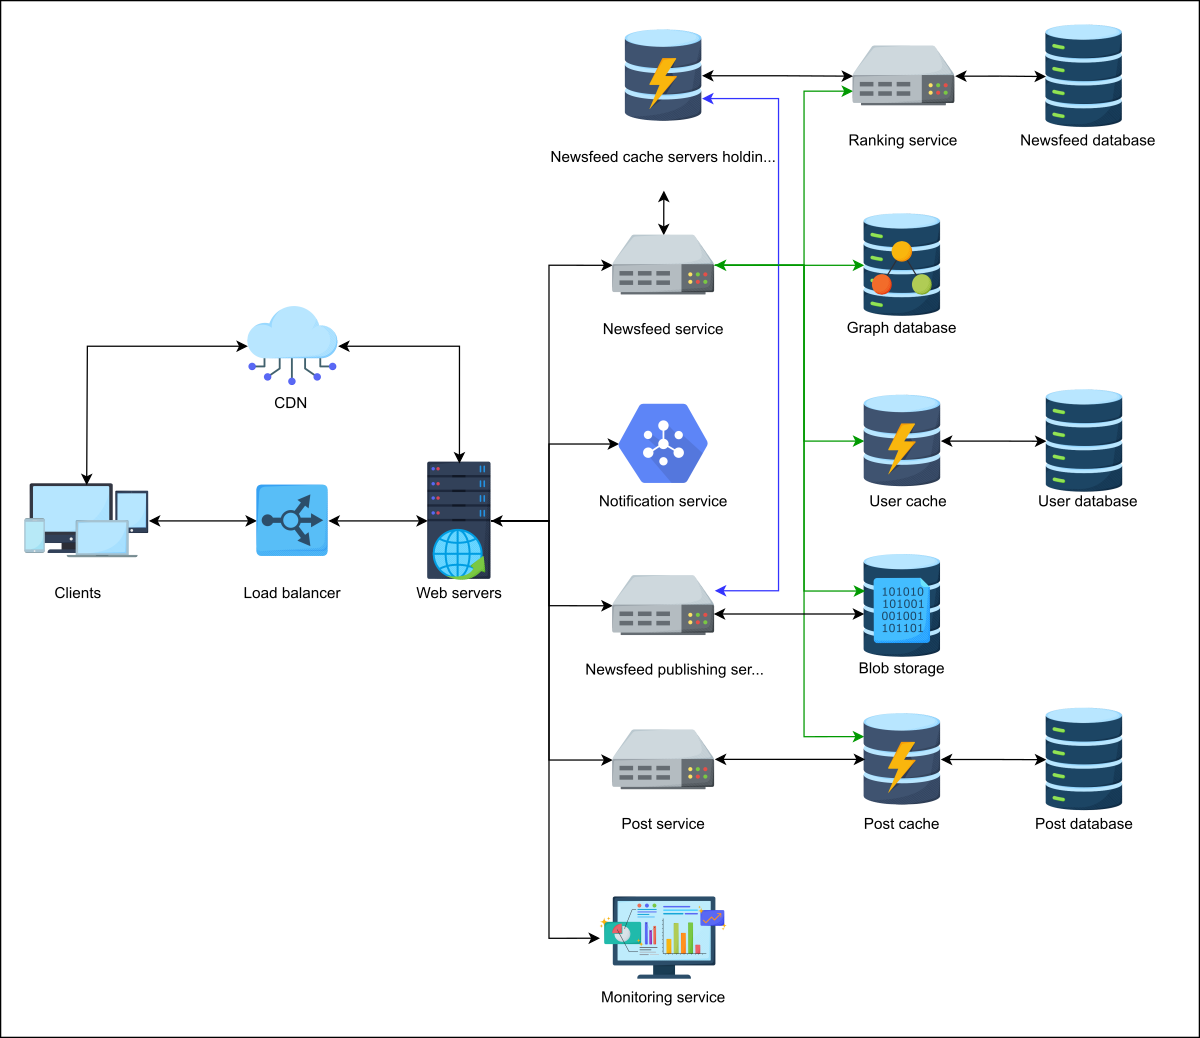
\includegraphics[width=0.5\textwidth]{Images/chapter_32/section_4943636425080832/5509169350574080.png}
 \caption{The detailed design of newsfeed system}
\end{figure}

With the full design established, the final step is validation. Let 's analyze the system to confirm its compliance with our requirements for scalability, availability, and low latency.

\subsection{Requirements compliance}\label{d25UkiRmKYPRTOddTVCKj}
\\
Our non-functional requirements for the proposed newsfeed System Design are scalability, fault tolerance, availability, and low latency. Let 's discuss how the proposed system fulfills these requirements:

\begin{enumerate}
\item
\protect\phantomsection\label{uRi0jGAoeQIK7LYFf4sjs}
\textbf{Scalability:} The proposed system is scalable to handle an ever-increasing number of users. The required resources, including load balancers, web servers, and other relevant servers, are added/removed on demand.
\item
\protect\phantomsection\label{CjfL70lJy2-nv22_H6Iw-}
\textbf{Fault tolerance}: The replication of data consisting of users' metadata, posts, and newsfeed makes the system fault-tolerant. Moreover, the redundant resources are always there to handle the failure of a server or its component. Monitoring service is used to enhance reliability by continuously observing system health, detecting issues early, providing insights for optimization, and assisting in timely incident response.
\item
\protect\phantomsection\label{0aXHmg9EAtg80KCglC4FG}
\textbf{Availability:} The system is highly available by providing redundant servers and replicating data on them. When a user gets disconnected due to some fault in the server, the session is re-created via a load balancer with a different server. Moreover, the data (users\textquotesingle{} metadata, posts, and newsfeeds) is stored on different and redundant database clusters, which provides high availability and durability.
\item
\protect\phantomsection\label{DoUMMj3kAp3gN9wm6xv9d}
\textbf{Low latency:} We can minimize the system's latency at various levels by:

\begin{enumerate}
\item
Geographically distributed servers and the cache associated with them. This way, we bring the service close to users.
\item
Using CDNs for frequently accessed newsfeeds and media content.
\end{enumerate}
\end{enumerate}
\\
Imagine you're the tech lead responsible for running a social media platform smoothly. We currently have 500 million daily active users, and this number is expected to double next year! To handle this surge, we need to improve the scalability of our Newsfeed system.
\\
Which approach would you prioritize to handle this increased user load?

\begin{enumerate}
\item
Add even more powerful servers to our infrastructure.
\item
Shard the data across multiple database instances.
\end{enumerate}
\\
Also, state the reason behind your choice.

\textbf{Question:}

Strategy for scaling the newsfeed design

\textbf{Reference Answer:}

Second option. Sharding the data across multiple database instances. Sharding is a better approach for handling increased user load because it offers scalability and redundancy, while adding more powerful servers creates a bottleneck and isn't sustainable in the long term.

\subsection{Quiz on the newsfeed system's design}\label{zied7TqpBt2--mcb9Felv}
\\
Test your understanding of the concepts related to the design of the newsfeed system with a quiz.

\subsection*{Quiz}
\vspace{0.3cm}
\noindent
\textbf{Question 1:} Which component is responsible for storing relationships between users, their friends, and followers?
\\[0.2cm]
\begin{itemize}
 \item The users database
 \item \textbf{[CORRECT]} The graph database
 \item The posts database
 \item None of the above
\end{itemize}
\vspace{0.3cm}
\noindent
\textbf{Question 2:} Where are fully constructed and ranked newsfeeds stored?
\\[0.2cm]
\begin{itemize}
 \item The published feeds cache
 \item \textbf{[CORRECT]} The newsfeed cache
 \item The posts cache
 \item None of the above
\end{itemize}
\vspace{0.3cm}
\noindent
\textbf{Question 3:} When do the web servers call the posts service?
\\[0.2cm]
\begin{itemize}
 \item \textbf{[CORRECT]} When new posts are created
 \item When a request for a newsfeed is received
 \item When users are to be notified due to some failure events
 \item All of the above
\end{itemize}
\vspace{0.3cm}
\noindent
\textbf{Question 4:} Which option below is stored in blob storage?
\\[0.2cm]
\begin{itemize}
 \item Comments on posts
 \item Count of likes and dislikes
 \item \textbf{[CORRECT]} Media content
 \item All of the above
\end{itemize}

\subsection{Summary}\label{D2pyuSJpL7NBk-90cWEYI}
\\
We learned to design a newsfeed system at scale. Our design ranked enormous user data to show carefully curated content to the user for a better user experience and engagement. Our newsfeed design is general enough that it can be used in many places, such as Twitter feeds, Facebook posts, YouTube and Instagram recommendations, News applications, and so on.

% End of section content